% !TEX root = ../main.tex
\section{Empirical Study}
\label{sec:hvm-experiments}
% !TEX root = ../main.tex
\begin{figure*}[t]
  \centering
  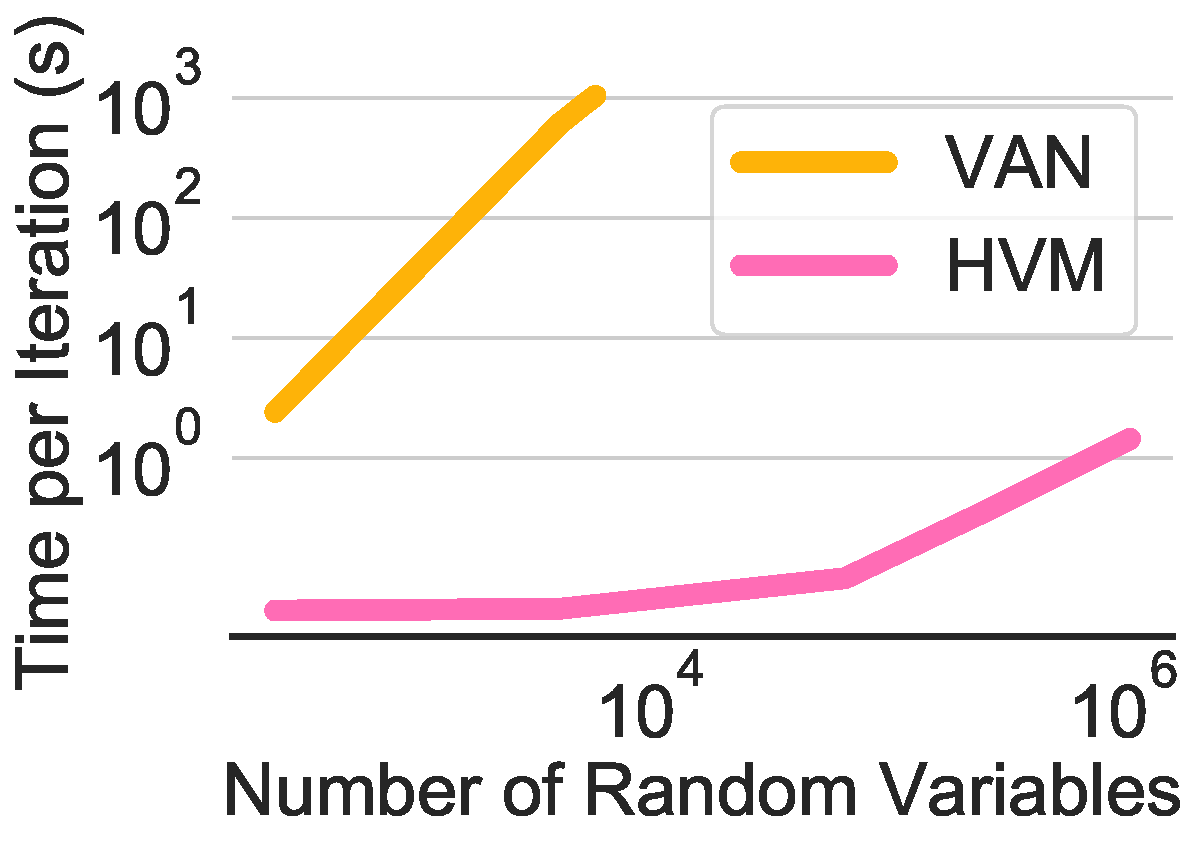
\includegraphics[width=0.5\textwidth]{fig/ising-scaling.pdf}
  \caption[Comparing scaling of \textsc{hvm}s to \textsc{van}s in large systems]{\textbf{\Acrfullpl{hvm} are faster than \Acrfullpl{van} \citep{wu2019solving} and scale to larger systems.} The scaling of both variational approximations is illustrated with the time taken per iteration in Ising models. The \gls{hvm} variational approximations use $5400$ parameters and the \gls{van} method uses over $700$k. The \gls{van} approximation runs out of memory with $16384$ random variables, while the \gls{hvm} method scales to models with over $1$M random variables.}
  \label{fig:ising-scaling}
\end{figure*}
To study the utility of \gls{vi} tools for statistical physics systems, we compare \glspl{hvm} to \gls{van} approximations~\citep{wu2019solving}.\footnote{Code is available at \url{https://github.com/altosaar/hierarchical-variational-models-physics}.} We use the same benchmarks as in \citet{wu2019solving}: the models of Ising and Sherrington-Kirkpatrick. We evaluate variational inference methods by assessing whether they lead to lower estimates of the free energy of a model. (Lower is better, as the free energy in  \Cref{eq:free-energy} is proportional to the negative of the variational lower bound in \Cref{eq:llbo,eq:hier-elbo}.)

\paragraph{Experimental Setup.} To assess whether \glspl{hvm} outperform \glspl{van} in large systems, the computational budget for the \gls{vi} algorithm using both variational approximations was set to 6~hours.  All experiments were performed on NVIDIA Tesla P100 GPUs, and the reference implementation of \glspl{van} released in \citet{wu2019solving} was used. \gls{van} models were unable to complete sufficiently many iterations in the allocated compute time, so all experiments were run without annealing the temperature of the system. For calculating the free energy using \glspl{hvm}, importance sampling~\citep{owen2013monte} was used with an \gls{hvm} as the proposal (for \glspl{van}, the increased cost of sampling prohibited drawing enough samples for low-variance importance sampling estimates, so Monte Carlo estimation was used). In \glspl{hvm}, variational approximations that accounted for problem structure using \gls{realnvp} transformations outperformed autoregressive parameterizations, and we omit these results.

\paragraph{Ising Model.} For small systems, \glspl{hvm} were more accurate than \gls{van} models at lower temperatures; at higher temperatures (such as the critical temperature), \gls{van} models were slightly more accurate. This could be because annealing was not used to fit \gls{van} models, and the randomness of the hierarchical latent variables in \glspl{hvm} obviates the need for annealing. In large systems (e.g. $L=128$), \gls{van} models failed to complete a single iteration, while \glspl{hvm} were able to complete many iterations (at the cost of some accuracy). The trade-off between model size and computational cost was significant between autoregressive choices of variational approximations in \glspl{hvm} versus \gls{realnvp} convolutional approximations. \Cref{fig:hvm-ising} shows that convolutional models were able to scale to models with over a million random variables, with only a slight decrease in accuracy relative to \gls{van} methods, and with $100$ times fewer parameters. This is also illustrated via the time per iteration for both a \gls{van} and \gls{hvm} variational approximation reported in \Cref{fig:ising-scaling}.

% !TEX root = ../../main.tex
\newcommand{\mysize}{0.2\textheight}
\newcommand{\mywidth}{0.1\linewidth}
\newcommand{\figwidth}{0.5\linewidth}
\begin{figure*}[t]
  \centering
  % adjust margin to center captions
  \captionsetup[subfigure]{margin={0cm,0cm},oneside}
  \hspace*{\fill}%
  \begin{subfigure}[c]{0.5\linewidth}
    \centering
    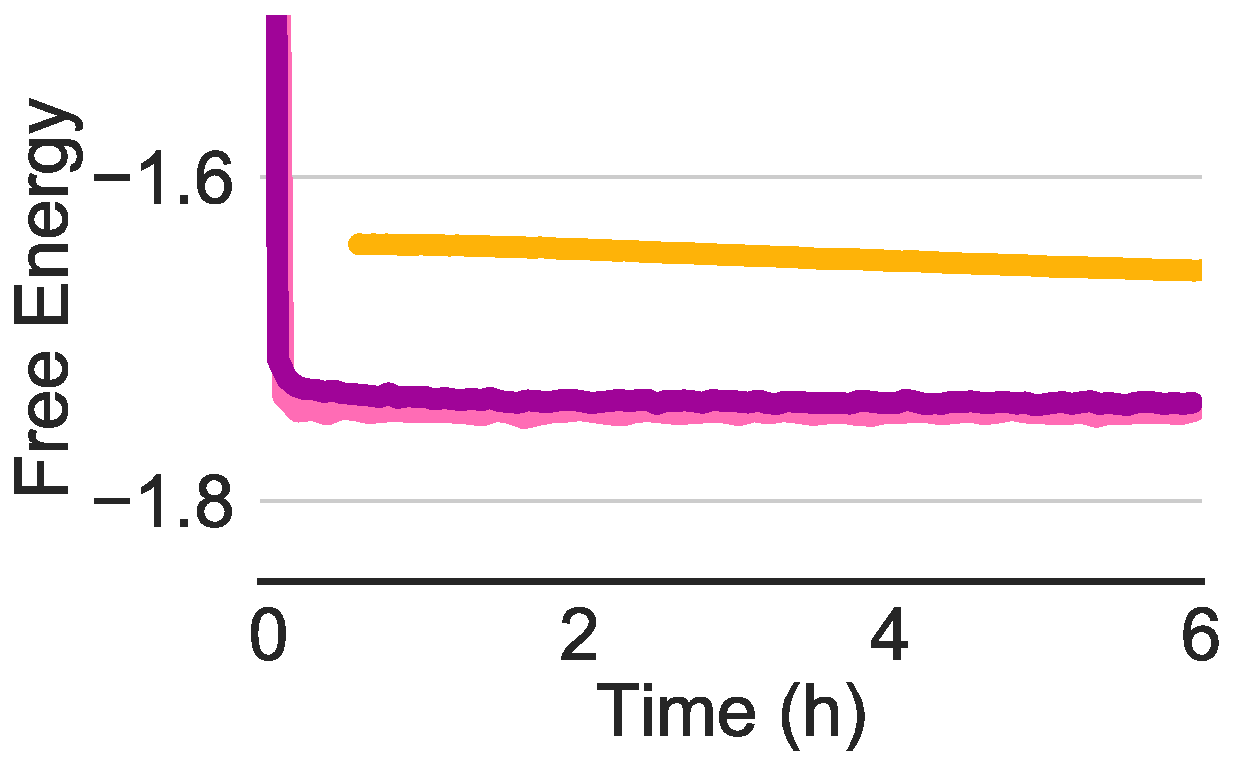
\includegraphics[width=\textwidth]{ch-hvm/fig/sk-large.pdf}
    % \caption{$\beta=0.4$}%
  \end{subfigure}
  % \hfill\hspace{\mywidth}%
  \begin{subfigure}[c]{0.3\linewidth}
    \centering
    % \raisebox{12mm}{
      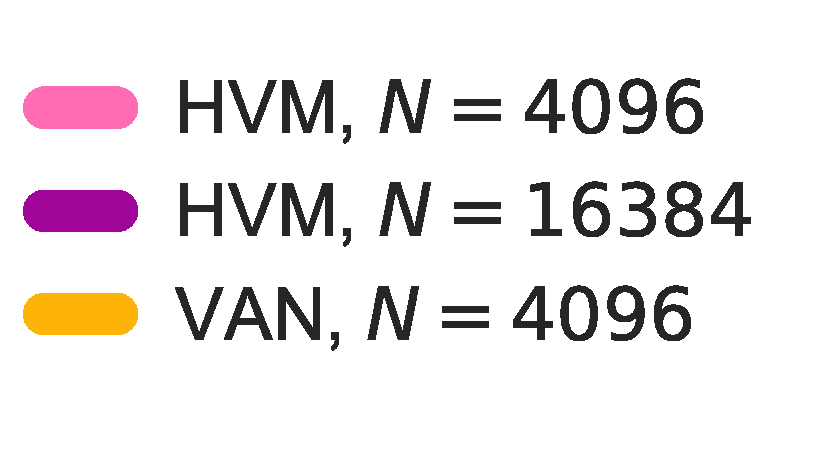
\includegraphics[width=\textwidth]{ch-hvm/fig/legend-sk}
    % }
  \end{subfigure}
  \hspace*{\fill}%
  % \vspace{-0.5cm}
  \caption[\textsc{hvm}s applied to the Sherrington-Kirkpatrick model]{\textbf{\Acrfullpl{hvm} scale to larger systems than \acrfull{van} models \citep{wu2019solving} when fit to the Sherrington-Kirkpatrick model using \acrlong{vi}.} (Lower is better, as the variational lower bound yields an upper bound on the free energy.) For the system with $N=4096$ variables the \gls{van} method completed fewer than ten iterations, and with $N=16384$ did not complete a single iteration.}
  \label{fig:sk}
\end{figure*}

\paragraph{Sherrington-Kirkpatrick Model.} The free energy estimates using \gls{vi} with either \gls{hvm} or \gls{van} approximations are plotted in \Cref{fig:sk} for the Sherrington-Kirkpatrick model. \gls{hvm} approximations outperformed \gls{van} approximations, and scaled to larger systems where the $\cO(L^2)$ cost of sampling from a \gls{van} prohibited even a single iteration.

\section{Discussion}
The \gls{gbf} inequality holds for quantum systems~\citep{feynman1972statistical,feynman2018statistical}, and  applying \gls{vi} and \glspl{hvm} to quantum systems is a direction for future work. Physics tools (such as \gls{vi} in its original incarnation) have been useful in machine learning~\citep{bamler2017perturbative}, and we hope the reverse holds---that tools from machine learning such as \gls{vi} and \glspl{hvm} continue to find use in statistical physics. Further scaling \glspl{hvm} to statistical physics models where system size is a bottleneck is a goal of future work, especially in settings relevant to medicine, such as in protein folding or drug screening problems.